
\chapter{同步性改善全局最优的递归自修复算法}

\section{自修复算法目标}
根据上文所述,当多机器人编队中度较高的机器人出现缺失时,会导致编队同步性下降。假设在图\ref{fig:修复路径对比}中,空缺位置表示出现机器人缺失,记缺失机器人为$R_f$,则缺失机器人的度$d_{R_f} = 6$。由引理\ref{lem:degree_syn}可知。若用度小于$d_{R_f}$的机器人修复此缺失机器人,则会提高编队的同步性。若最终修复机器人为$R_r$,度为$d_{R_r}$。则$d_{R_f}-d_{R_r}$的值越大,同步性改善效果越好。因此,如果用编队中度最小的机器人去修复缺失机器人则会使同步性改善效果最优。
\begin{figure}[!htbp]
	\centering
	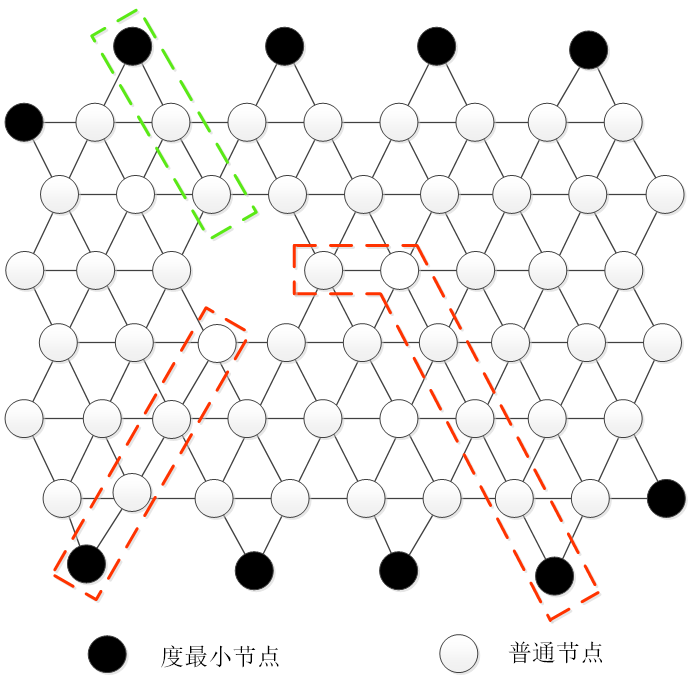
\includegraphics[width=8cm,height=8cm]{chapter3/figure3-1.png}
	\bicaption[fig:修复路径对比]{不同修复路径对比}{不同修复路径对比}{Fig}{The comparation of different repairing paths.}
\end{figure}

如何找到一条从缺失机器人到度最小机器人的修复路径是本文算法的主要内容。在这里修复路径定义为从缺失机器人邻居中的某个机器人到编队中度最小机器人所经过的机器人序列$\{R_1,R_2,\dots,R_{k-1},R_k\}$。修复路径上的机器人成为修复机器人,其中$R_1$为缺失机器人邻居中的某个机器人,$R_k$为编队中某个度最小的机器人。在图\ref{fig:修复路径对比}中,每一个虚线框中的机器人序列都属于一条修复路径。从图中可以看到不同的修复路径包含的修复机器人个数不同。定义包含修复机器人个数最少的修复路径为最优修复路径,图中绿色虚线框内的修复路径即为一条最优修复路径。如果一条修复路径中的修复机器人序列为$\{R_1,R_2,\dots,R_{k-1},R_k\}$,则对应的递归自修复步骤如下:\\
\indent (1)从缺失机器人的邻居中选择一个修复机器人$R_1$,$R_1$去填补缺失机器人留下的空缺位置,并与缺失机器人邻居重新建立。\\
\indent (2)$R_1$从其邻居中选择一个修复机器人$R_2$用来填补$R_1$移动后留下的空缺位置,并与$R_1$的邻居重新建立连接。\\
\indent (3)重复上述过程,直到编队中的度最小机器人$R_k$填补了$R_{k-1}$留下的空缺位置。\\
第(3)步结束后,整个修复机器人序列的递归自修复过程结束。在这一过程中,修复机器人的空间位置和网络邻居变化如下:\\
空间位置变化:\\
\begin{equation}
	P_{R_i} = 
	\begin{cases}
		P_{R_f}, & i=1 \\
		P_{R_{i-1}}, & 1 < i \leq k
	\end{cases}
\end{equation}
网络邻居变化:\\
\begin{equation}
	N_e(R_i) = 
	\begin{cases}
		N_e(R_f) - R_i + R_{i+1}, & i = 1 \\
		N_e(R_{i-1}) - R-i + R_{i+1}, & 1<k \leq k
	\end{cases}
\end{equation}

由于本文采用递归自修复方式实现分布式控制,因此编队中机器人无法知道距离缺失机器人最近的度最小机器人在哪里。即如何找到一条最优的修复路径?